\begin{figure}
	
	\floatbox{figure}[\FBwidth]
	{
		\caption{Distribution of review times at \textit{Econometrica}}\label{figure5}
	}
	{
		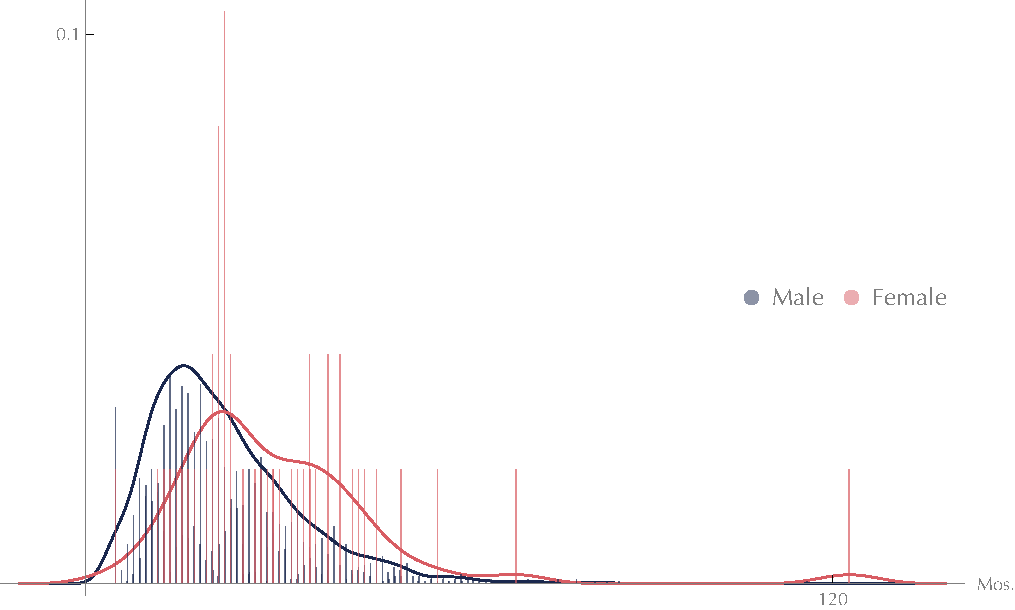
\includegraphics[width=12.3cm]{$HOME/Dropbox/Readability/draft/pdf/figure5.pdf}
		\floatfoot{\tiny \textit{Notes}. Sample 2,446 articles. Bars are proportional to the number of papers published in \textit{Econometrica} with a given review time (months between first submission and final acceptance). Blue bars represent papers written only by men (2,397); pink bars are papers written only by women (49). Source: \textit{Econometrica}.}
	}
\end{figure}